%% LyX 2.3.1-1 created this file.  For more info, see http://www.lyx.org/.
%% Do not edit unless you really know what you are doing.
\documentclass[english,hebrew]{article}
\usepackage[T1]{fontenc}
\usepackage[utf8]{inputenc}
\usepackage{babel}
\usepackage{amstext}
\usepackage{graphicx}
\usepackage[unicode=true]
 {hyperref}
\begin{document}
\title{מה זה לוגריתמים ובשביל מה זה טוב?}
\maketitle
\begin{description}
\item [{קטגוריות:}] כללי
\item [{תגים:}] לוגריתמים
\item [{מזהה:}] \L{what\_are\_logarithms}
\end{description}
מבין כל המושגים במתמטיקה שנלמדים בבית הספר, לוגריתמים הם כנראה המושג
שנשכח הכי בקלות והכי פחות ברור בשביל מה הוא טוב, בעצם. זה כמובן חבל
מאוד כי זה מושג מגניב מאוד )וגם שימושי, אבל לא בחיי היום יום שלנו
ואני לא אנסה לטעון אחרת( והוא גם לא קשה כל כך להבנה. אני אתחיל מלהסביר
מה זה בעצם, ואז נדבר על הבשביל-מה-זה-טוב.

התשובה הקצרה היא \textquotedblright לוגריתם זו הפעולה ההפוכה לחזקה
כמו שחיסור הוא הפעולה ההפוכה לחיבור וחילוק הוא הפעולה ההפוכה לכפל\textquotedblleft{}
אבל העלילה מסתבכת כבר בשלב הזה, כי יש \textbf{שתי} פעולות הפוכות לחזקה
ששונות אחת מהשניה מאוד, כי בניגוד לחיבור וכפל, חזקה היא לא פעולה \textbf{סימטרית}.
מבלבל? כן, אז בואו נתחיל מההתחלה.

אני מניח שאנחנו מכירים חיבור - זו נקודת התחלה לא רעה. אנחנו יודעים
ש-\L{$3+5=5+3$} )זה \textbf{חוק החילוף}(. אנחנו יודעים שחיסור הוא
פעולה הפוכה לחיבור במובן הבא: \L{$3+5-5=3$}. כלומר, אם חיברתי ל-{\beginL 3\endL}
ואז חיסרתי ממנו את אותו מספר, אז אני אחזור אל מה שהתחלתי ממנו. אני
רוצה טיפה לחדד את זה בצורה שנשמעת פדנטית אבל בהמשך אולי יהיה ברור
למה אני מתעקש עליה: הפעולה \textquotedblright לחסר {\beginL 5\endL}\textquotedblleft{}
היא הפעולה ההפוכה של \textquotedblright לחבר {\beginL 5\endL}\textquotedblleft .
כמובן שלא נכון לומר ש\textquotedblleft לחסר {\beginL 5\endL}\textquotedblleft{}
היא הפעולה ההפוכה של \textquotedblright לחבר {\beginL 4\endL}\textquotedblleft ,
כלומר יש חשיבות לשאלה מה המספר הספציפי שמחסרים.

עכשיו נעבור אל פעולת הכפל. מה זה כפל? סביר שגם אותו אנחנו מכירים:
על כפל במספר טבעי אפשר לחשוב בתור הרבה פעולות חיבור. \L{$3\times5$}
הוא דרך אחרת לומר \L{$3+3+3+3+3$} - חיברנו את {\beginL 3\endL} לעצמו
{\beginL 5\endL} פעמים. עכשיו, עבור כפל, קורה אותו הסיפור שקרה עבור
חיבור בדיוק: \L{$3\times5=5\times3$} - הנה שוב חוק החילוף בפעולה.
והפעולה ההפוכה ל\textquotedblleft כפל ב-{\beginL 5\endL}\textquotedblleft{}
נקראת \textquotedblright חלוקה ב-{\beginL 5\endL}\textquotedblleft{}
ואני לרוב מסמן אותה ככה: \L{$3\times5\times\frac{1}{5}=3$} )כלומר,
אני \textbf{מגדיר} חלוקה ב-{\beginL 5\endL} בתור כפל ב-\L{$\frac{1}{5}$}(.
ההבדל היחיד בין חיבור וחיסור ובין כפל וחילוק הוא שבכפל וחילוק, לא
קיימת פעולה הפוכה ל\textquotedblleft כפל ב-{\beginL 0\endL}\textquotedblleft .
אבל זה \L{\href{https://gadial.net/2008/10/16/nullity_part_1/}{סיפור לפעם אחרת}}.

אחרי כפל, הפעולה הבאה שאפשר לדבר עליה היא \textbf{חזקה}. אם כפל במספר
טבעי מוגדר בתור \textquotedblright לחזור על החיבור כמה פעמים\textquotedblleft ,
אז העלאה בחזקת מספר טבעי מוגדרת בתור \textquotedblright לחזור על הכפל
כמה פעמים\textquotedblleft . כלומר, הסימון \L{$3^{5}$} מייצג את \L{$3\times3\times3\times3\times3$}
- כופלים את {\beginL 3\endL} בעצמו {\beginL 5\endL} פעמים.

וכאן הסיפור מתחיל להסתבך.

בניגוד לחיבור וכפל, חוק החילוף \textbf{לא מתקיים} עבור חזקות. אפשר
פשוט לבדוק את זה בעזרת דוגמא: \L{$3^{5}=243$} אבל \L{$5^{3}=125$}.
המקרה היחיד של שני מספרים שונים זה מזה שעבורם חוק החילוף מתקיים הוא
\L{$2^{4}=4^{2}=16$} )ואיכשהו אלו תמיד שני המספרים הראשונים שעולים
לי לראש כשאני רוצה לתת דוגמאות לחזקה(. גם הכתיב של חזקה מאפשר לנו
לראות שאין סימטריה: בביטוי \L{$3^{5}$} יש את המספר שכתוב בגדול ואת
זה שנמצא בקטן למעלה. למספר הגדול שלמטה, {\beginL 3\endL} במקרה שלנו,
קוראים \textbf{בסיס החזקה}. למספר הקטן שלמעלה, {\beginL 5\endL} במקרה
הנוכחי, קוראים \textbf{מעריך החזקה}. פעולת החזקה פירושה לכפול את בסיס
החזקה שוב ושוב בעצמו מספר פעמים ששווה למעריך החזקה.

אם כן, העלאה בחזקה היא פעולה שכוללת שני \textquotedblright קלטים\textquotedblleft{}
שונים. נוח לדבר על הפעולה הזו כש\textquotedblleft מקפיאים\textquotedblleft{}
את אחד מהקלטים להיות איזה שהוא ערך קונקרטי ואז שואלים את עצמו מה קורה
כשנותנים ערכים שונים ומשונים בתור הקלט השני. קשר כזה בין קלטים ופלטים
נקרא \textquotedblright פונקציה\textquotedblleft .

בואו נראה דוגמא קונקרטית. נניח שנקפיא את \textbf{מעריך} החזקה להיות
תמיד {\beginL 2\endL}, ונשאל את עצמנו מה קורה עבור בסיסים שונים. נקבל
את הפונקציה \L{$f\left(x\right)=x^{2}$} שאנחנו קוראים לה \textbf{העלאה
בריבוע}. הפעולה ה\textquotedblleft הפוכה\textquotedblleft{} להעלאה
בריבוע היא הוצאת שורש ריבועי: \L{$g\left(x\right)=\sqrt{x}$}. אני
כותב \textquotedblright הפוכה\textquotedblleft{} במרכאות כי זה לא מדויק
במאה אחוזים: אם אני לוקח את \L{$-2$} ומעלה אותו בריבוע אקבל {\beginL 4\endL},
ואחרי הוצאת שורש ריבועי אקבל {\beginL 2\endL} כי מגדירים את פעולת
הוצאת השורש ככזו שמחזירה את השורש החיובי.

באופן דומה אפשר לדבר על העלאה בחזקות גבוהות יותר: \L{$f\left(x\right)=x^{n}$}
עבור \L{$n$} טבעי כלשהו. הפעולה ההפוכה לזה נקראת \textquotedblright שורש
מסדר גבוה\textquotedblleft{} ומסומנת ב-\L{$g\left(x\right)=\sqrt[n]{x}$}.
את הפעולות הללו אנחנו מכירים יחסית טוב; למשל, הקפיצה מאורך צלע של
קוביה אל הנפח שלה היא העלאה בחזקה שלישית, ולכן הקפיצה חזרה מנפח של
קובייה אל אורך הצלע שלה הוא הוצאת שורש שלישי. כמובן, במכולת אנחנו
לא זקוקים לפעולות הללו אבל הן יותר נטועות במציאות היומיומית שלנו מאשר
מה שאנחנו הולכים לדבר עליו עכשיו.

עכשיו, סוף כל סוף, אנחנו מגיעים אל לוגריתמים.

ראשית, בואו נדבר על הפעולה של העלאה בחזקה כשדווקא \textbf{הבסיס} קבוע.
בואו נקבע אותו להיות מספר שרירותי כלשהו, נאמר {\beginL 10\endL} כי
אנחנו אוהבים את {\beginL 10\endL}. אז יש לנו את הפונקציה \L{$f\left(x\right)=10^{x}$}.
הפונקציה הזו נקראת \textbf{פונקציה אקספוננציאלית} והיא אחת מהפונקציות
שמצטלמות הכי גרוע שאפשר:

\L{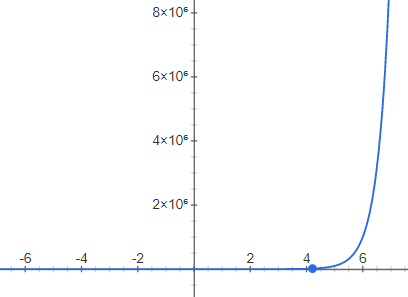
\includegraphics{C:/Users/gadia/Dropbox/Websites/blog/assets/img/2020/06/exponential.PNG}}

לוגריתם הוא ההפך מהפונקציה האקספוננציאלית הזו: \L{$\log\left(10^{x}\right)=x$}.
באופן כללי: \L{$\log$} על קלט \L{$y$} כלשהו בודק מהו ה-\L{$x$}
שעבורו \L{$10^{x}=y$}, ואז הוא מחזיר את ה-\L{$x$} הזה. הוא עונה
על השאלה \textquotedblright{\beginL 10\endL} בחזקת איזה מעריך נותן
לנו את \L{$y$}?\textquotedblleft{}

אז כדי לראות כמה דוגמאות: \L{$\log\left(10\right)=1$} ו-\L{$\log\left(1000\right)=3$}
ו-\L{$\log\left(10000000\right)=6$} ו-\L{$\log\left(1\right)=0$}
כי \L{$10^{0}=1$} )כי \L{\href{https://gadial.net/2018/01/01/zero_power_equals_one/}{דברים בחזקת 0 שווים 1}}(.
כאן אנחנו רואים משהו חשוב על לוגריתמים: זו פונקציה שגדלה \textbf{לאט}.
כדי לקבל ערכים יותר ויותר גדולים של לוגריתם, צריך להזין קלטים \textbf{הרבה
יותר גדולים}. 

ומה עם \L{$\log\left(121\right)$}, למשל? לכמה זה שווה? אם תבדקו במחשבון
הוא יגיד משהו בסגנון \L{$\log\left(121\right)=2.08278\ldots$}. זה
קצת מוזר, כי עד עכשיו בפוסט הזה לא דיברנו בכלל על חזקות שהן לא מספר
טבעי. מה זה \L{$10^{2.08278\ldots}$}? זה לכפול את {\beginL 10\endL}
בעצמו פעמיים ואז... לעשות... מה בעצם?

בואו ניקח, אם כן, צעד אחד אחורה וננסה להבין קצת יותר טוב איך הולך
כל העניין הזה עם חזקות - כי אחרי שנבין אותו, נבין מצויין גם מה הולך
עם לוגריתמים.

בואו ניקח בסיס חזקה קבוע שהוא מספר חיובי, שאני אסמן באות \L{$a$}
כי אין לי כוח לכתוב \L{$10$} או משהו דומה כל הזמן. בואו ניקח עכשיו
שתי חזקות שונות של \L{$a$}: \L{$a^{x},a^{y}$} ו\textbf{נכפול} אותן.
מה נקבל? אם \L{$x,y$} הם מספרים טבעיים ואנחנו הולכים על פי ההגדרה
של \textquotedblright חזקה היא ביצוע של אותה פעולת כפל שוב ושוב\textquotedblleft{}
קל לראות ש-\L{$a^{x}\cdot a^{y}=a^{x+y}$} )שימו לב שהתחלתי לתאר כפל
עם נקודה ולא עם \L{$\times$} סתם כי זה סימון שיותר נוח לי(. באופן
דומה לא קשה לראות ש-\L{$\left(a^{x}\right)^{y}=a^{xy}$}. במילים אחרות:
פעולת החזקה איכשהו מתרגמת את פעולת \textbf{החיבור }של המעריכים לפעולת
\textbf{כפל }של תוצאות החזקה, ואת פעולת \textbf{הכפל} של המעריכים
לפעולת העלאה בחזקה נוספת של פעולת החזקה. זה כל כך חשוב שאני אכתוב
את זה שוב במפורש:
\begin{itemize}
\item \L{$a^{x+y}=a^{x}\cdot a^{y}$}
\item \L{$a^{xy}=\left(a^{x}\right)^{y}$}
\end{itemize}
ההגדרה של פעולת החזקה לחזקות שהן לא מספרים טבעיים לוקחת את המשוואות
הללו בתור נקודת המוצא ושואלת את השאלה - אם אני רוצה שהן ימשיכו להתקיים
גם אחרי שנרשה ל-\L{$x,y$} להיות מספרים לא טבעיים, מה חייב לקרות?

אז למשל, אם \L{$y=0$}, השוויון \L{$a^{x+0}=a^{x}\cdot a^{0}$} מתורגם
ל-\L{$a^{x}=a^{x}\cdot a^{0}$} מה ש\textquotedblleft מכריח\textquotedblleft{}
את \L{$a^{0}=1$}. ועכשיו, \L{$a^{x+\left(-x\right)}=a^{x}\cdot a^{-x}$}
מתורגם ל-\L{$1=a^{x}\cdot a^{-x}$} מה ש\textquotedblleft מכריח\textquotedblleft{}
את \L{$a^{-x}=\frac{1}{a^{x}}$} )זה לא עובד אם \L{$a=0$}! לכן אני
דורש ש-\L{$a$} יהיה מספר חיובי!(. כמו כן, מכיוון ש-\L{$\frac{1}{2}+\frac{1}{2}=1$}
אז \L{$a=a^{1}=a^{\frac{1}{2}+\frac{1}{2}}=\left(a^{\frac{1}{2}}\right)^{2}$}
\textquotedblright מכריח\textquotedblleft{} את \L{$a^{\frac{1}{2}}=\sqrt{a}$}
ובאופן כללי יותר מקבלים \L{$a^{\frac{1}{n}}=\sqrt[n]{a}$}. מכל אלו
אנחנו מקבלים את ההגדרה \L{$a^{\frac{x}{y}}=\sqrt[y]{a^{x}}$} שעובדת
למעריך שהוא מספר רציונלי כללי )מספר רציונלי הוא מספר שהוא מנה של שני
מספרים שלמים, \L{$\frac{x}{y}$}(.

השלב האחרון, של להגדיר חזקה שהיא לא מספר רציונלי אלא מספר ממשי כללי,
היא מסובכת יותר פשוט כי ההגדרה של \textquotedblright מספר ממשי כללי\textquotedblleft{}
היא מסובכת. אני יכול לומר ש-\L{$a^{x}$} מוגדר בתור \L{$\lim_{q\to x}a^{q}$}
כך ש-\L{$q$} היא סדרת רציונליים ששואפת ל-\L{$x$}, אבל זה לא יגיד
כלום אם לא מכירים את המושגים הרלוונטיים וגם אם מכירים אותם יש כל מני
שאלות מציקות )למה זה אותו גבול עבור כל סדרת רציונליים?( אז אני לא
אכנס לזה הפעם, אבל זה עובד יפה.

עכשיו נחזור לדבר על לוגריתמים. ראשית כל, עד עכשיו דיברתי על לוגריתם
שהיה קשור למספר {\beginL 10\endL}, אבל אין משהו קדוש ב-{\beginL 10\endL};
גם מספרים אחרים יכולים להיות בסיס ללוגריתם. למשל {\beginL 2\endL}:
אפשר לדבר על \L{$\log_{2}$} שמוגדר כך: אם \L{$y=2^{x}$} אז \L{$\log_{2}y=x$}.
יש ל-\L{$\log_{2}$} הזה אפילו סימון מיוחד: \L{$\lg$}. ואפשר לעשות
את אות והדבר גם עבור בסיסים אחרים. המגבלה שאנחנו דורשים היא שהבסיס
יהיה מספר גדול מ-{\beginL 1\endL}, כי עבור {\beginL 1\endL} העסק כבר
מתחיל להיות מעצבן )מכיוון שלכל \L{$x$} מתקיים \L{$1^{x}=1$} יוצא
ש-\L{$\log$} על בסיס {\beginL 1\endL} לא מוגדר לשום מספר שונה מ-{\beginL 1\endL}(
וגם עבור מספרים קטנים ממנו העסק בעייתי בצורות דומות. לכן דורשים \L{$1<a$}
ואז אפשר לדבר על \L{$\log_{a}$}, שמוגדרת כפי שכבר ראינו: אם \L{$y=a^{x}$}
אז \L{$\log_{a}\left(y\right)=x$}. כלומר, יש הרבה סוגים שונים של
לוגריתמים, כפי שיש הרבה סוגים שונים של שורשים )ריבועי, שורש שלישי
וכן הלאה(.

למעשה, הבסיס \textbf{הכי חשוב} של הלוגריתם הוא בכלל לא מספר טבעי אלא
מספר שמסומן ב-\L{$e$} ושווה בערך ל-\L{$2.7182\ldots$} )זה לא מספר
רציונלי ולכן אין מחזוריות בספרות(. מה זה המספר הזה? למה הוא חשוב כל
כך? \L{\href{https://gadial.net/2010/03/27/exponent/}{יש לי פוסט}}
שמציג אותו בצורה שנראית לי טבעית יחסית, אבל לא ניכנס לכך בפוסט הנוכחי
- ההסבר המדויק מערב, כרגיל, חשבון דיפרנציאלי ואינטגרלי. גם ל-\L{$\log_{e}$}
יש סימון מיוחד: \L{$\ln$} )ולפעמים אפילו כותבים פשוט \L{$\log$}
למרות שמתכוונים אל \L{$\ln$}(, אבל לא ארחיב על כך יותר בפוסט הזה.

עכשיו, אם נסתכל שניה על מחשבון, נראה שאין בו הרבה כפתורים עבור לוגריתמים.
אם יש לנו מזל יש אחד עבור \L{$\log$} ואחד עבור \L{$\ln$} וזהו זה.

\L{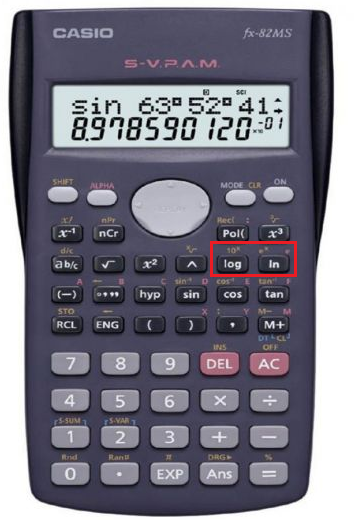
\includegraphics{C:/Users/gadia/Dropbox/Websites/blog/assets/img/2020/06/calc.PNG}}

איך אפשר לחשוב לוגריתמים עבור בסיסים אחרים? למרבה המזל, יש קשר הדוק
בין לוגריתמים בבסיסים שונים שמאפשר לנו לחשב את \L{$\log_{a}b$} גם
אם כל מה שיש לנו הוא \L{$\log$} רגיל על בסיס {\beginL 10\endL} )או
עבור כל בסיס אחר(.

התעלול עובד כך: נניח ש-\L{$x=\log_{a}b$}, ונחפש דרך נחמדה לבטא את
\L{$x$} באמצעות \L{$\log$} רגיל, על בסיס {\beginL 10\endL}. מכיוון
ש-\L{$x=\log_{a}b$} אז \textbf{על פי ההגדרה ממש} אנחנו יודעים ש-\L{$a^{x}=b$}.

עכשיו, לתעלול! כל עוד \L{$a>1$}, אפשר להוכיח )שוב, זה דורש חדו\textquotedblleft א(
ש-\L{$t=\log a$} הוא מספר שבאמת קיים. כלומר, שקיים \L{$t$} כלשהו
כך ש-\L{$a=10^{t}$}. כשאנחנו מצויידים בידע הזה בואו נחזור למשוואה
\L{$a^{x}=b$} ונציב \L{$10^{t}$} במקום \L{$a$}. נקבל:

\L{$b=a^{x}=\left(10^{t}\right)^{x}=10^{tx}$}

כשהמעבר האחרון נובע מחוקי החזקות שהראיתי קודם.

עכשיו, מה המשמעות של השוויון \L{$b=10^{tx}$}? כמקודם, \textbf{על
פי ההגדרה ממש} משמעותו היא \L{$\log b=tx$}. או במילים אחרות, \L{$x=\frac{\log b}{t}$}.
אבל מה היה \L{$t$}? לכו טיפה אחורה ותראו ש-\L{$t=\log a$}. כלומר
קיבלנו \L{$x=\frac{\log b}{\log a}$}, ובמילים אחרות: \L{$\log_{a}b=\frac{\log b}{\log a}$}.
כך אפשר לחשב לוגריתם על פי כל בסיס בעזרת מחשבון שיודע רק לחשב את \L{$\log$}
על בסיס {\beginL 10\endL}.

למעשה, אנחנו רואים כאן אפילו טיפה יותר מכך: אם נגדיר פונקציה \L{$f\left(x\right)=\log_{a}x$},
אנחנו רואים ש-\L{$f\left(x\right)=\frac{1}{\log a}\log x$}. במילים
אחרות, ההבדל בין פונקציית הלוגריתם \textquotedblright הרגילה\textquotedblleft ,
על בסיס {\beginL 10\endL}, ובין כל פונקציית לוגריתם אחרת הוא רק \textbf{כפל
בקבוע}. זו תוצאה מעניינת מאוד כשאנחנו במדעי המחשב, למשל, ואנחנו מתעניינים
רק בסדרי גודל של דברים ולא בערך המספרי המדויק שלהן; זה אומר שכל הפונקציות
הלוגריתמיות הן \textbf{מאותו סדר גודל.}

עכשיו, אחרי שהבנו מה זה לוגריתמים, בואו ננסה לראות בשביל מה זה טוב.
בשביל זה כדאי לראות עוד תכונות שלוגריתמים מקיימים. נתחיל עם יישום
של הנוסחה \L{$\log_{a}b=\frac{\log b}{\log a}$} שראינו עבור מקרה
פרטי. אם \L{$b=a^{x}$}, אז \L{$x=\log_{a}b=\frac{\log\left(a^{x}\right)}{\log\left(a\right)}$}.
אם נכפול את שני קצוות המשוואה ב-\L{$\log\left(a\right)$} נקבל \L{$\log\left(a^{x}\right)=x\log\left(a\right)$}.
זו תכונה חשובה של לוגריתם - הוא \textquotedblright מוריד את המעריך\textquotedblleft{}
מחזקה והופך אותו לכפל; זה בעצם ההופכי של תכונת ה-\L{$a^{xy}=\left(a^{x}\right)^{y}$}
של הפונקציה המעריכית, שבה כפל הופך לחזקה.

באופן דומה גם לתכונת ה\textquotedblleft חיבור הופך לכפל\textquotedblleft ,
\L{$a^{x+y}=a^{x}\cdot a^{y}$}, יש היפוך: \L{$\log_{a}x+\log_{a}y=\log_{a}\left(xy\right)$}.
כדי לראות את זה אני הולך להיעזר בעוד תכונה פשוטה של לוגריתמים: \L{$a^{\log_{a}x}=x$}.
כלומר, לוגריתם בתוך מעריך של חזקה מתבטל עם החזקה; זו פחות או יותר
ההגדרה. הרי אמרנו ש-\L{$\log_{a}x=t$} פירושו ש-\L{$a^{t}=x$}, אז
אם נכתוב את \L{$\log_{a}x$} במקום \L{$t$} נקבל בדיוק \L{$a^{\log_{a}x}=x$}.

עכשיו בואו נוכיח את התכונה על סכום הלוגריתמים. לשם כך, בואו נתקע את
הסכום בתוך המעריך של חזקה:

\L{$a^{\log_{a}x+\log_{a}y}=a^{\log_{a}x}\cdot a^{\log_{a}y}=x\cdot y$}

כאשר המעבר הראשון נובע מהתכונה של אקספוננטים להפוך סכום למכפלה, והמעבר
השני הוא ה-\L{$a^{\log_{a}x}=x$} שהראיתי. עכשיו אפשר לקחת את \L{$xy$}
ולהשתמש עליו באותה נוסחה: \L{$xy=a^{\log_{a}\left(xy\right)}$}. קיבלנו
בסך הכל:

\L{$a^{\log_{a}x+\log_{a}y}=a^{\log_{a}\left(xy\right)}$}

עכשיו נפעיל את \L{$\log_{a}$} על שני האגפים ונקבל \L{$\log_{a}\left(x\right)+\log_{a}\left(y\right)=\log_{a}\left(xy\right)$},
כפי שרצינו.

הנוסחה הזו חשובה. \textbf{ממש חשובה}. עד כמה חשובה? חשובה ברמה של
להשפיע על כל ההיסטוריה האנושית. אבל למה? כי פעם, חברות וחברים, לא
היו מחשבונים. כשאנשים רצו לחשב משהו, הם היו צריכים \textbf{לחשב} אותו.
נניח, צריך לכפול שני מספרים גדולים, כי למשל אתם ימאים וצריכים לחשב
מסלול וזה מאוד חשוב כדי לא להתרסק עם סלעים? עדיף שתעשו את זה \textbf{מדויק}.
הצורך הזה בדיוק אצל ימאים הוביל להמצאת שעונים סופר-מדויקים שעבדו גם
בים, וזה סיפור מרתק בפני עצמו; אז גם שיטות חישוב מדויקות זה דבר חשוב.

עכשיו, להכפיל שני מספרים גדולים זה לא \textbf{כזה} קשה, אבל זה גם
לא קל - תנסו לכפול שני מספרים של {\beginL 10\endL} ספרות כל אחד ומהר
מאוד תראו שזו הרבה עבודה, והסכנה לטעות היא גדולה. מה שיפה בלוגריתמים
זה שהם יכולים לחסוך חלק נכבד מהעבודה כי הם \textbf{ממירים בעיה של
כפל בבעיה של חיבור}.

הנה שיטת העבודה: נניח שיש לי מספרים \L{$x,y$} ואני רוצה לחשב את \L{$xy$}
בקלות. מה אעשה? ראשית כל, אחשב את \L{$\log\left(x\right),\log\left(y\right)$};
עכשיו אבצע פעולת \textbf{חיבור} שתיתן לי את \L{$\log\left(x\right)+\log\left(y\right)=\log\left(xy\right)$}.
עכשיו רק צריך לשחזר מתוך \L{$\log\left(xy\right)$} את \L{$xy$} ו...
ניצחנו! איזה יופי! רק שאלה קטנה נשארה: איך, בהינתן \L{$x,y$}, מחשבים
מתוכם את \L{$\log\left(x\right)$} ואת \L{$\log\left(y\right)$}?
ואיך מתוך \L{$\log\left(xy\right)$} מקבלים חזרה את \L{$xy$}? התשובה
היא כמובן... מחשבון! רגע, משהו לא מסתדר פה.

אפשר לחשב לוגריתמים גם בלי מחשבון, אבל זו יכולה להיות עבודה קשה למדי.
הנקודה היא שזו עבודה שמספיק לבצע \textbf{פעם אחת}, ואז לכתוב את כל
התוצאות בטבלה יפה, ואז להפיץ את הטבלה הזו באינסוף עותקים ברחבי העולם,
וכולם יוכלו להשתמש בה. זה היה הרעיון מאחורי טבלות הלוגריתמים שערכו
במאה ה-{\beginL 17\endL} ג'ון נפייר והנרי בריגס.

\L{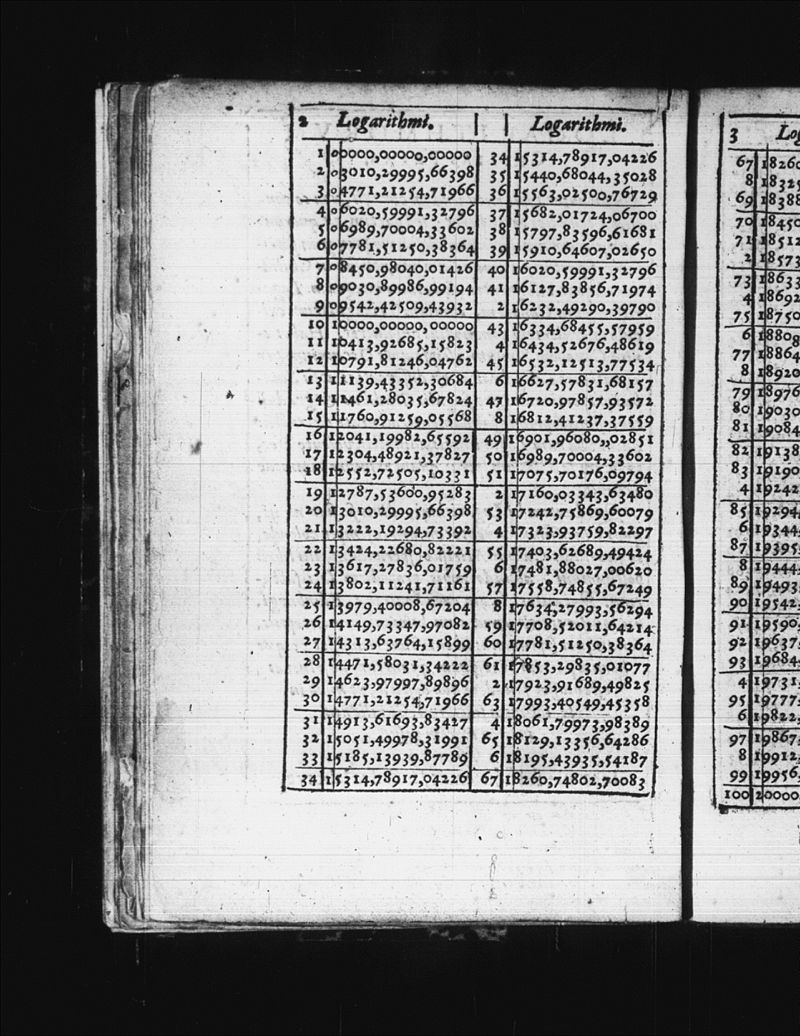
\includegraphics{C:/Users/gadia/Dropbox/Websites/blog/assets/img/2020/06/logarithms}}

אני מתחמק כאן מכניסה לפרטים הטכניים של איך להשתמש בטבלאות הללו כי
הפוסט ממילא ארוך מדי, אבל הרעיון ברור - בעזרת הטבלאות היה אפשר לחשב
יחסית בקלות לוגריתמים, מה שאיפשר למי שיש לו טבלה כזו להמיר כפל בחיבור.
באופן דומה גם אפשר היה להמיר חילוק בחיסור, כי מתקיים גם הכלל הבא:
\L{$\log_{a}x-\log_{a}y=\frac{x}{y}$}. כדי לראות את זה אפשר להשתמש
בכללים שכבר ראינו: ראינו ש-\L{$\log_{a}x^{t}=t\log_{a}x$}, ולכן בפרט
עבור \L{$t=-1$} נקבל \L{$-\log_{a}x=\log_{a}x^{-1}=\log_{a}\frac{1}{x}$},
ומכאן נשתמש בכלל החיבור עבור \L{$\log_{a}x-\log_{a}y=\log_{a}x+\left(-\log_{a}y\right)$}.

כדי לפשט את העניינים אף יותר, הומצא גם מכשיר שנקרא \textquotedblright סרגל
חישוב\textquotedblleft{} שדומה לסרגל רגיל פרט לכך שהסקלות שעליו הן
לוגריתמיות. גם לו מגיע פוסט משל עצמו )שאני תמיד מתכנן ואף פעם לא כותב(
ולא אתעכב עליו הפעם.

\L{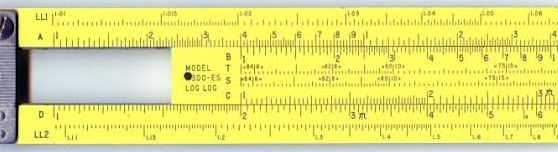
\includegraphics{C:/Users/gadia/Dropbox/Websites/blog/assets/img/2020/06/Pocket_slide_rule}}

אם כן, ראינו את השימוש ה\textquotedblleft היסטורי\textquotedblleft{}
החשוב של לוגריתמים. אבל בימינו יש מחשבונים וכבר לא צריך את הלוגריתמים
לשם כך. האם אפשר לשכוח מהם לחלוטין?

ובכן, במתמטיקה בוודאי שאין סיבה לשכוח מהם. הם היו ונותרו כלי עזר מאוד
מועילים בהתמודדות עם בעיות מסויימות, בזכות התכונות הנחמדות של המרת-כפל-לחיבור
והורדת-חזקה-למטה. לוגריתם הוא כלי בסיסי בארגז הכלים של מתמטיקאי שעוסק
באנליזה של ביטוי מסובך כלשהו, אבל אני לא אדבר על זה יותר מדי כאן.
שאלה קצת יותר מעניינת היא האם לוגריתמים רלוונטיים איכשהו בחיי היום
יום שלנו. והתשובה היא - במיוחד כיום, לצערי כן.

למה \textquotedblright לצערי\textquotedblleft ? כי הדוגמא הראשונה
שקופצת לי לראש היא זו של מגיפת הקורונה של {\beginL 2020\endL}.

הבה ונסתכל בגרף של מספר מקרי הקורונה בעולם בין ינואר ליוני {\beginL 2020\endL}:

\L{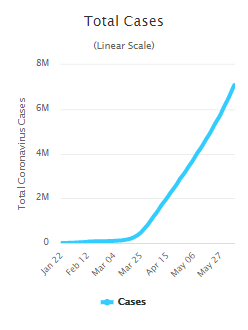
\includegraphics{C:/Users/gadia/Dropbox/Websites/blog/assets/img/2020/06/corona-linear.PNG}}

מה זה גרף, בעצם? לכל תאריך בטווח התאריכים המדובר, נצבעה נקודה כחולה
שקואורדינטת ה-\L{$x$} שלה )המיקום שלה מבחינת ימין/שמאל( היא התאריך
הזה, וקואורדינטת ה-\L{$y$} שלה )הגובה שלה( מתאימה למספר החולים באותו
תאריך. אחר כך כל הנקודות חוברו זו לזו בצורה שמאפשרת לראות בקלות את
קו המגמה. זה גרף מעניין כי הוא מתחיל אקספוננציאלי - יש קפיצה אדירה
באיזור חודש מרץ - ואז משנה מגמה והופך ללינארי )כלומר, נראה כמו קו
ישר(.

המשמעות של גידול אקספוננציאלי היא זו: שאם מחלקים את הגידול לפרקי זמן
קצרים, אז בכל פרק זמן הגידול \textbf{כפול} ממה שהיה קודם )כפול בקבוע
כלשהו,לאו דווקא ב-{\beginL 2\endL}(. זה מאופיין על ידי פונקציה כמו
\L{$f\left(t\right)=a^{t}$} )כאן \L{$t$} הוא הזמן(. המשמעות של גידול
לינארי היא שאם מחלקים את הגידול לפרקי זמן קצרים, אז בכל פרק זמן הגידול
זהה למה שהיה קודם - למשל \L{$f\left(t\right)=at$}. את החלק הלינארי
אפשר לראות די בבירור, אבל הקפיצה האקספוננציאלית היא פשוט קפיצה: נראה
שהגרף \textquotedblright שטוח\textquotedblleft{} ברגע אחד, ופתאום הוא
מתחיל לעלות - שינוי שמעביר אותו מאפס למיליון כמעט בבת אחת.

אבל יש דרך אחרת להציג את הנתונים, שעוזרת להבין אותם יותר טוב - סקלה
\textbf{לוגריתמית}. מה זה אומר? ובכן, בסקלה רגילה, לינארית, הגובה
של ערך בציר \L{$y$} הוא פונקציה לינארית של הערך שלו. אם נסתכל על
הגרף שלמעלה, נראה שערכים של {\beginL 2\endL} מיליון מפוזרים במרווחים
שווים. אם \L{$f$} היא הפונקציה שמתאימה לערך את הגובה שלו אז \L{$f\left(2\cdot10^{6}\right)=a$}
כאשר \L{$a$} הוא הגובה של הקו הראשון, זה שכתוב לידו \L{$\text{2M}$};
ואז \L{$f\left(4\cdot10^{6}\right)=2a$} ו-\L{$f\left(6\cdot10^{6}\right)=3a$}
וכן הלאה: הפונקציה באופן כללי היא \L{$f\left(x\right)=\frac{a}{2\cdot10^{6}}x$}.
זו דוגמא לפונקציה לינארית - היא לוקחת את \L{$x$} וכופלת אותו בקבוע.

הנה איך אותו גרף נראה בסקלה לוגריתמית:

\L{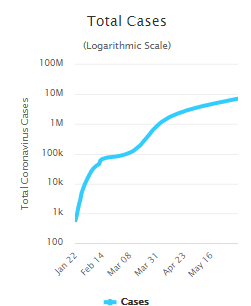
\includegraphics{C:/Users/gadia/Dropbox/Websites/blog/assets/img/2020/06/corona-log.PNG}}

מה השתנה? ציר \L{$y$}. אם נסתכל על הערכים שם, נראה שעכשיו מה שקורה
במרווחים שווים הוא שהערך שמיוצג \textbf{מוכפל ב-}\textbf{{\beginL 10}\endL}.
הערך הנמוך ביותר הוא {\beginL 100\endL}; אחר כך, במרווח שווה ממנו,
יש את \L{$1,000$}; אחר כך במרווח שווה ממנו יש את \L{$10,000$} וכן
הלאה. אם נסמן את הגובה של הקו של ה-{\beginL 1,000\endL} ב-\L{$a$}
אז נקבל את הפונקציה \L{$f\left(x\right)=\log\left(x\right)a-2a$}
)ה-\L{$-2a$} מגיע מכך שהקו התחתון בגרף, זה שבגובה {\beginL 0\endL},
הוא {\beginL 100\endL}(.

דרך ההתבוננות הזו על הנתונים מאפשרת לנו לראות בצורה יותר טובה מה קרה
באיזור של מרץ, שבגרף הלינארי פשוט נראה כמו קפיצה אדירה: אנחנו רואים
שהעלייה כמעט נפסקה לתקופה כלשהי ואז התחדשה במלוא המרץ )זה קרה כשהוירוס
התחיל להתפשט באירופה וארה\textquotedblleft ב(. זו דוגמא קטנה לשימושיות
של סקלות לוגריתמיות.

יש עוד סקלות לוגריתמיות שמשמשות אותנו בחיי היום יום - מדידה של חומציות
עם סקלת \L{pH} היא לוגריתמית; מדידה של רעש עם סקלת הדציבלים היא לוגריתמית,
ואולי הסקלה הלוגריתמית המוכרת ביותר היא סולם ריכטר למדידת העוצמה של
רעידות אדמה. כשמדווחים על רעידות אדמה בדרך כלל אומרים שהן היו בעוצמה
של \textquotedblright{\beginL 5.8\endL} בסולם ריכטר\textquotedblleft{}
או \textquotedblright{\beginL 6.1\endL} בסולם ריכטר\textquotedblleft{}
וכדומה. אל תתנו למספרים הדומים לבלבל אתכם - כל עליה בסולם ריכטר פירושה
\textbf{הכפלה} בקבוע כלשהו של עוצמת רעידת האדמה. רעידת אדמה שהיא {\beginL 3\endL}
בסולם ריכטר בקושי תורגש; רעידת האדמה של יפן ב-{\beginL 2011\endL}
שהייתה {\beginL 9\endL} בסולם ריכטר לא הייתה פי {\beginL 3\endL} יותר
מה\textquotedblleft בקושי תורגש\textquotedblleft{} הזה אלא הייתה אסון
אדיר ממדים וחריג בעוצמתו.

הייתי רוצה לסיים כאן את הפוסט, אבל הוא לקח כיוון אפל מאוד לקראת סופו
- מגיפות, רעידות אדמה... הלוגריתמים האומללים שבסך הכל רצו לעזור לנו
לכפול ולחלק מעורבים בזוועות הללו בגלל היכולת שלהם לתאר לנו דברים בקנה
מידה \textbf{גדול}, כולל אסונות. אז אני רוצה לסיים דווקא בגישה האופטימית
- זמן ריצה של אלגוריתמים.

בלי להיכנס לעובי הקורה של איך מודדים זמן ריצה של אלגוריתמים, הרעיון
הוא שאם יש לנו מספר \L{$n$} שמהווה מדד כלשהו לגודל של הקלט, ויש לנו
פונקציה \L{$f\left(n\right)$} שאומרת לנו מה הולך להיות זמן הריצה
על קלט בגודל \L{$n$} במקרה הגרוע ביותר, אז אנחנו מתעניינים במה סדר
הגודל \textbf{בערך} של \L{$f$} הזו. \L{\href{https://gadial.net/2012/07/06/asymptotic_notation/}{יש לי פוסט}}
שמסביר את הסימון שבו משתמשים למטרה הזו אבל אין צורך לקרוא אותו כרגע:
הרעיון הוא שאם אני כותב \L{$f\left(n\right)=O\left(n^{2}\right)$},
למשל, זה אומר שאני יכול להבטיח ש-\L{$f$} היא לא יותר מאשר בערך הפונקציה
\L{$n^{2}$}.

בעיה בסיסית במדעי המחשב היא בעיה של \textbf{מיון}. נניח שיש לנו קבוצה
של \L{$n$} מספרים ואני רוצה לסדר אותם בסדר עולה. כמה זמן יידרש לי
לשם כך? שיטות נאיביות כמו לקחת איבר ולהשוות אותו לכל האיברים שסידרנו
עד כה כדי לדעת איפה לדחוף אותו )שיטה שנקראת \textbf{מיון הכנסה} ודומה
לאופן שבו מסדרים קלפים ביד במשחק קלפים( לוקחות לי בערך \L{$O\left(n^{2}\right)$}
זמן. זה לא טוב. תחשבו על סיטואציה עם {\beginL 1000\endL} קלטים - זמן
הריצה יהיה בערך {\beginL 1,000,000\endL} )מיליון מה? כאמור, אני מטאטא
את הפרטים מתחת לשטיח(. ואם אני מכפיל את מספר הקלטים ב-{\beginL 10\endL},
אז זמן הריצה גדל פי {\beginL 100\endL}. זה בהחלט לא משהו.

אבל יש מיונים יותר מתוחכמים ויותר מהירים, למשל \L{\href{https://gadial.net/2012/07/10/all_sorts_of_slow_sorts/}{מיון מיזוג}}.
מבלי להיכנס לפרטים, הרעיון במיון הזה הוא לחלק את הקבוצה שצריך למיין
לשני חלקים. ואז כל חלק למיין לשני חלקים. ושוב, ושוב, עד שמגיעים לקבוצות
קטנות מספיק כדי שאפשר יהיה למיין אותן \textquotedblright מייד\textquotedblleft{}
ואז מתחילים למזג בצורה חכמה את הקבוצות הממויינות. והרי לכם שאלה: נניח
שיש לי \L{$n$} איברים ובכל סיבוב אני מחלק את קבוצות האיברים שלי ל-{\beginL 2\endL};
כמה סיבובים יידרשו עד שקבוצות האיברים שלי יהיו מגודל אפסי?

נניח שהקבוצה שלי היא בת {\beginL 16\endL} איברים. אחרי סיבוב אחד אקבל
שתי קבוצות של {\beginL 8\endL} איברים; אחרי {\beginL 2\endL} סיבובים
הקבוצות יהיו בנות {\beginL 4\endL} איברים ואחרי {\beginL 3\endL} סיבובים
הן יהיו בנות {\beginL 2\endL} איברים. אחרי {\beginL 4\endL} סיבובים
הן יהיו בנות {\beginL 4\endL} איברים ואפשר יהיה לסיים כאן. כל סיבוב
הקטין את גודל הקבוצה פי {\beginL 2\endL}, כלומר כפל אותה בחצי: אם
\L{$n$} הוא הגודל המקורי של הקבוצה אז אחרי \L{$k$} סיבובים נקבל
קבוצות בנות \L{$\frac{n}{2^{k}}$} איברים. אם \L{$\frac{n}{2^{k}}=1$}
אז \L{$n=2^{k}$}, כלומר \L{$k=\lg n$} )כזכור, \L{$\lg$} הוא לוגריתם
על בסיס {\beginL 2\endL}(. אם כן, מספר הצעדים עד שמגיעים לקבוצות קטנות
הוא \textbf{לוגריתמי} ב-\L{$n$}. זה אומר שגם כאשר \L{$n$} הוא \textbf{ממש
גדול}, מספר הצעדים עד לפיצול יהיה ממש קטן. המשך הניתוח של האלגוריתם
יראה שבהתחשב בזמן שלוקח לבצע את המיזוג, זמן הריצה הכולל של האלגוריתם
יהיה \L{$O\left(n\log n\right)$}, וזאת להבדיל מהאלגוריתמים של \L{$O\left(n^{2}\right)$}.
הדבר הזה הוא \textbf{שיפור גדול}, כי \L{$\log n$} הרבה יותר קטן מ-\L{$n$}
ולכן \L{$n\log n$} הרבה יותר קטן מ-\L{$n^{2}$}. למשל, עבור \L{$n=1000$},
ראינו ש-\L{$n^{2}=1,000,000$} בעוד ש-\L{$n\log n=3000$}.

והנה עוד דוגמא אחרונה לסיום - מספרים גדולים. אנחנו מתעסקים עם מספרים
גדולים כל הזמן - דוגמא פופולרית במיוחד היא שיטת ההצפנה \L{$\text{RSA}$}
שמתבססת על עבודה עם מספרים בני מאות ספרות. אנחנו צריכים לבצע איתם
פעולות כמו חיבור, כפל, העלאה בחזקה וכדומה; כמה זמן זה לוקח?

ובכן, התשובה טמונה במה שאמרתי במשפט הקודם: כשאני מדבר על \textquotedblright מספר
בן מאות ספרות\textquotedblleft{} המשמעות היא \textquotedblright מספר
שהלוגריתם שלו הוא בסדר גודל של כמה מאות\textquotedblleft . הלוגריתם
בבסיס {\beginL 10\endL} של מספר כלשהו הוא פשוט מספר הספרות שלו פחות
{\beginL 1\endL} ועוד תיקון כלשהו. למשל, עבור \L{$100$} הלוגריתם
הוא בדיוק {\beginL 2\endL}, ואילו עבור {\beginL 121\endL} ראינו שהלוגריתם
הוא \textquotedblright{\beginL 2\endL} ועוד קצת משהו\textquotedblleft{}
שהוא פחות ממספר שלם.

עכשיו, אלגוריתמים עבור חיבור וכפל, גם מאלו שלומדים בבית הספר היסודי,
הם משהו שעובד \textbf{על הספרות} של המספר. למשל, אלגוריתם לחיבור מחבר
ספרה-ספרה, החל מספרת האחדות. אז הזמן שאלגוריתמים כאלו לוקחים הוא מסדר
גודל של לוגריתם של המספר, או ריבוע של לוגריתם כזה, וכו; כלומר משהו
כמו \L{$O\left(\log^{2}n\right)$} כדי לבצע כפל. כשמתעסקים במספרים,
אלו זמני הריצה שנחשבים יעילים; זמן ריצה של \L{$O\left(n\right)$}
הוא אסון, כי אם \L{$n=10^{100}$} למשל )וזה מספר קטן יחסית למספרים
שאנחנו עשויים להתעסק איתם( אז פרק זמן ששווה בערך ל-\L{$10^{100}$}
הוא גדול בהרבה מהשניות שחלפו מאז תחילת היקום.

לסיכום, ראינו לוגריתמים וראינו קצת איך הם רלוונטיים לדברים במתמטיקה;
אני מקווה שעכשיו הם מפחידים או מסתוריים קצת פחות, כי בסך הכל הם חברים
די טובים שלנו.
\end{document}
